

\tikzset{every picture/.style={line width=0.75pt}} %set default line width to 0.75pt        

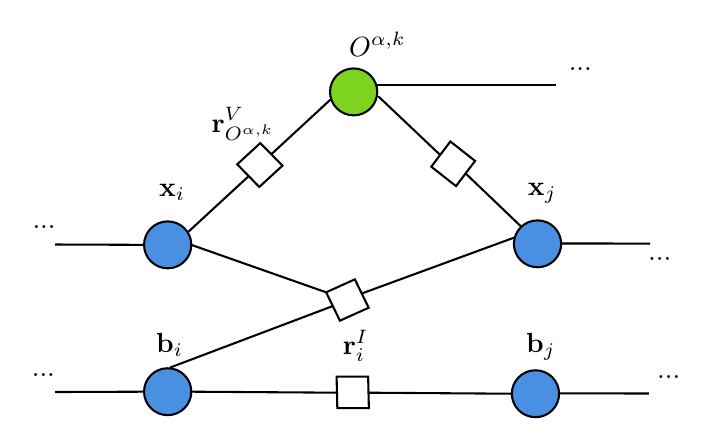
\begin{tikzpicture}[x=0.75pt,y=0.75pt,yscale=-0.7,xscale=0.7]
%uncomment if require: \path (0,300); %set diagram left start at 0, and has height of 300

%Shape: Ellipse [id:dp45734499228140624] 
\draw  [fill={rgb, 255:red, 74; green, 144; blue, 226 }  ,fill opacity=1 ] (173.77,161.65) .. controls (173.77,152.74) and (181.05,145.51) .. (190.04,145.51) .. controls (199.02,145.51) and (206.3,152.74) .. (206.3,161.65) .. controls (206.3,170.57) and (199.02,177.8) .. (190.04,177.8) .. controls (181.05,177.8) and (173.77,170.57) .. (173.77,161.65) -- cycle ;
%Shape: Ellipse [id:dp47015016474354476] 
\draw  [fill={rgb, 255:red, 74; green, 144; blue, 226 }  ,fill opacity=1 ] (428.33,160.95) .. controls (428.33,152.04) and (435.61,144.81) .. (444.59,144.81) .. controls (453.57,144.81) and (460.85,152.04) .. (460.85,160.95) .. controls (460.85,169.87) and (453.57,177.09) .. (444.59,177.09) .. controls (435.61,177.09) and (428.33,169.87) .. (428.33,160.95) -- cycle ;
%Shape: Ellipse [id:dp9295682874620682] 
\draw  [fill={rgb, 255:red, 74; green, 144; blue, 226 }  ,fill opacity=1 ] (173.77,262.72) .. controls (173.77,253.8) and (181.05,246.58) .. (190.04,246.58) .. controls (199.02,246.58) and (206.3,253.8) .. (206.3,262.72) .. controls (206.3,271.64) and (199.02,278.86) .. (190.04,278.86) .. controls (181.05,278.86) and (173.77,271.64) .. (173.77,262.72) -- cycle ;
%Shape: Ellipse [id:dp6555143846606085] 
\draw  [fill={rgb, 255:red, 126; green, 211; blue, 33 }  ,fill opacity=1 ] (301.76,56.37) .. controls (301.76,47.46) and (309.04,40.23) .. (318.02,40.23) .. controls (327,40.23) and (334.28,47.46) .. (334.28,56.37) .. controls (334.28,65.29) and (327,72.52) .. (318.02,72.52) .. controls (309.04,72.52) and (301.76,65.29) .. (301.76,56.37) -- cycle ;
%Straight Lines [id:da9521520713119127] 
\draw [color={rgb, 255:red, 0; green, 0; blue, 0 }  ,draw opacity=1 ]   (204.41,152.53) -- (245.52,114.61) ;
%Shape: Rectangle [id:dp3161705184765987] 
\draw  [color={rgb, 255:red, 0; green, 0; blue, 0 }  ,draw opacity=1 ][fill={rgb, 255:red, 255; green, 255; blue, 255 }  ,fill opacity=1 ] (237.86,106.23) -- (253.8,91.61) -- (269.03,107.16) -- (253.09,121.79) -- cycle ;
%Straight Lines [id:da3213081425167289] 
\draw    (261.07,99.57) -- (301.99,61.75) ;
%Straight Lines [id:da6438250845761921] 
\draw [color={rgb, 255:red, 0; green, 0; blue, 0 }  ,draw opacity=1 ]   (334.99,59.42) -- (376.95,99.19) ;
%Shape: Rectangle [id:dp7790581824994257] 
\draw  [color={rgb, 255:red, 0; green, 0; blue, 0 }  ,draw opacity=1 ][fill={rgb, 255:red, 255; green, 255; blue, 255 }  ,fill opacity=1 ] (384.58,90.52) -- (401.61,103.89) -- (388.48,121.23) -- (371.46,107.86) -- cycle ;
%Straight Lines [id:da30524145360098653] 
\draw    (394.86,112.29) -- (433.51,149.25) ;
%Shape: Ellipse [id:dp05153463819108772] 
\draw  [fill={rgb, 255:red, 74; green, 144; blue, 226 }  ,fill opacity=1 ] (426.91,264.12) .. controls (426.91,255.21) and (434.2,247.98) .. (443.18,247.98) .. controls (452.16,247.98) and (459.44,255.21) .. (459.44,264.12) .. controls (459.44,273.04) and (452.16,280.27) .. (443.18,280.27) .. controls (434.2,280.27) and (426.91,273.04) .. (426.91,264.12) -- cycle ;
%Straight Lines [id:da17853834379013955] 
\draw [color={rgb, 255:red, 0; green, 0; blue, 0 }  ,draw opacity=1 ]   (206.3,262.72) -- (307.65,263.42) ;
%Shape: Rectangle [id:dp9066403918223247] 
\draw  [color={rgb, 255:red, 0; green, 0; blue, 0 }  ,draw opacity=1 ][fill={rgb, 255:red, 255; green, 255; blue, 255 }  ,fill opacity=1 ] (306.29,252.32) -- (328,252.37) -- (328.5,274.05) -- (306.79,274) -- cycle ;
%Straight Lines [id:da03645804386903806] 
\draw    (328.39,263.42) -- (426.91,264.12) ;
%Straight Lines [id:da027077311980835073] 
\draw [color={rgb, 255:red, 0; green, 0; blue, 0 }  ,draw opacity=1 ]   (191.69,246.11) -- (304.35,203.53) ;
%Shape: Rectangle [id:dp24365007507301994] 
\draw  [color={rgb, 255:red, 0; green, 0; blue, 0 }  ,draw opacity=1 ][fill={rgb, 255:red, 255; green, 255; blue, 255 }  ,fill opacity=1 ] (299.08,194.32) -- (318.85,185.41) -- (328.37,204.94) -- (308.59,213.84) -- cycle ;
%Straight Lines [id:da2648472917538476] 
\draw    (323.68,195.11) -- (428.33,156.74) ;
%Straight Lines [id:da14052768409961358] 
\draw [color={rgb, 255:red, 0; green, 0; blue, 0 }  ,draw opacity=1 ]   (206.3,161.65) -- (299.08,194.32) ;
%Straight Lines [id:da6158943819099749] 
\draw    (112.49,161.42) -- (173.77,161.65) ;
%Straight Lines [id:da9772427491569776] 
\draw    (112.49,262.95) -- (173.77,262.72) ;
%Straight Lines [id:da5013062146145252] 
\draw    (521.22,263.96) -- (459.94,263.89) ;
%Straight Lines [id:da11536516883313996] 
\draw    (522.16,160.78) -- (460.88,160.71) ;
%Straight Lines [id:da14002584664448192] 
\draw    (334.05,51.93) -- (457.55,51.93) ;

% Text Node
\draw (182.04,117.76) node [anchor=north west][inner sep=0.75pt]   [align=left] {$\displaystyle \mathbf{x}_{i}$};
% Text Node
\draw (435.88,117.06) node [anchor=north west][inner sep=0.75pt]   [align=left] {$\displaystyle \mathbf{x}_{j}$};
% Text Node
\draw (179.91,220.23) node [anchor=north west][inner sep=0.75pt]   [align=left] {$\displaystyle \mathbf{b}_{i}$};
% Text Node
\draw (312.83,12.89) node [anchor=north west][inner sep=0.75pt]   [align=left] {$\displaystyle O^{\alpha ,k}$};
% Text Node
\draw (218.11,64.93) node [anchor=north west][inner sep=0.75pt]   [align=left] {$\displaystyle \mathbf{r}_{O^{\alpha ,k}}^{V}$};
% Text Node
\draw (434.68,220.23) node [anchor=north west][inner sep=0.75pt]   [align=left] {$\displaystyle \mathbf{b}_{j}$};
% Text Node
\draw (308.4,218.26) node [anchor=north west][inner sep=0.75pt]   [align=left] {$\displaystyle \mathbf{r}_{i}^{I}$};
% Text Node
\draw (94.86,146.13) node [anchor=north west][inner sep=0.75pt]   [align=left] {...};
% Text Node
\draw (94.38,248.14) node [anchor=north west][inner sep=0.75pt]   [align=left] {...};
% Text Node
\draw (538.78,174.33) node [anchor=north west][inner sep=0.75pt]  [rotate=-180.29] [align=left] {...};
% Text Node
\draw (463.96,37.58) node [anchor=north west][inner sep=0.75pt]   [align=left] {...};
% Text Node
\draw (524.77,249.54) node [anchor=north west][inner sep=0.75pt]   [align=left] {...};


\end{tikzpicture}
